     \chapter{Stuff you want to include}
     \label{app:C}
     
	\subsection{Calculation of transducer RC circuit}
	\label{app:matlab}
R1 = \SI{500}{k\Omega}. $\tau = RC$. The capacitor charge oscillates between $V_L$ and $V_H$. $V_H =$ \SI{2.5}{V}. $V_L$ is reached for the first time at $t_{L_1}$ and $V_H$ at $t_{H_1}$. $V_L$ is then reached at  $t_{L_2}$. For \SI{150}{BPM} (or \SI{2.5}{Hz}), the pulse drives high for \SI{0.2}{ms}. Since the capacitor has to charge faster than \SI{0.2}{ms}, a charge time of \SI{0.16}{ms} was selected to add a 20\% margin, accounting for noise. Thus $t_{H_1} - t_{L_1} = 0.16$ and $t_{L_2} - t_{H_1} = 0.4 - 0.16 = 0.24$ for the 150 BPM signal. Finally,

$$V_L = 5\left(1-e^{\frac{t_{L_1}}{\tau}}\right)$$
$$V_H = 5\left(1-e^{\frac{-t_{H_1}}{\tau}}\right)$$
$$V_L = V_H\left(e^{\frac{t_{L_1}}{\tau}}\right)$$

giving $C = 1\mu$, when solving using the following MatLab script:\\

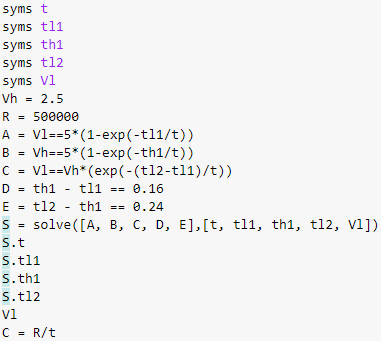
\includegraphics[width = 0.75\textwidth]{./Figures/script}

%	\subsection{Voltage Buffer}
%It is a good design practice to include a unity gain op-amp to acts as a voltage buffer by clamping $V_{in-}$ against fluctuations. This design practice was considered, but ultimately rejected, as tests with and without the buffer provided outputs of equal quality. This is the case as the signal conditioning circuit already has a very high input resistance. The only notable differences resulting from the inclusion of a buffer were an increase in current drawn, as well as an increase in cost for the circuit components, as another op-amp is required. Therefore, in order to keep the current consumption below \SI{15}{mA}, as well as to use reduce cost by only using three op-amps, the voltage buffer was omitted in the final design.